\documentclass[a4paper, oneside, 12pt, english]{article}
\usepackage{geometry}
\geometry{
	a4paper,
	total={154mm,227mm},
	left=28mm,
	top=35mm,
}
\setlength{\parskip}{0.85em}
\setlength{\parindent}{2.6em}
\usepackage{array}
\usepackage{amssymb}
\usepackage{enumerate}
\usepackage{graphicx}
\usepackage{url}
\usepackage{color}
\usepackage{wrapfig}
\usepackage{systeme}
\usepackage{tabularx}
\usepackage{subfig}
\usepackage{hyperref}
\usepackage[authoryear, round]{natbib}
\usepackage[dvipsnames]{xcolor}



\begin{document}
\begin{titlepage}
	\newcommand{\HRule}{\rule{\linewidth}{0.5mm}}
	\center
	\textsc{\LARGE Université de Liège}\\[1cm]
	\textsc{\Large Faculté des Sciences Appliquées}\\[2cm]
		
	\HRule \\[0.5cm]
	{ \huge \bfseries Automatic Multispeaker Voice Cloning}\\[0.2cm]
	\HRule \\[2cm]

	\begin{minipage}{0.4\textwidth}
		\begin{flushleft} \Large
			\emph{Author:}\\
			Corentin \textsc{Jemine}
		\end{flushleft}
	\end{minipage}
	~
	\begin{minipage}{0.4\textwidth}
		\begin{flushright} \Large
			\emph{Supervisor:} \\
			Prof. Gilles \textsc{Louppe}
		\end{flushright}
	\end{minipage}\\[4cm]
	
	{\LARGE Academic year 2018 - 2019}\\[1cm]
	
	
\includegraphics{images/uliege_logo.jpg}\\[1.25cm]
	
	\textit{Graduation studies conducted for obtaining the Master's degree \\in Data Science by Corentin Jemine}
	
	\vfill
\end{titlepage}
\setcounter{page}{2}

%\color{red}
%Possibly, start with a TTS lexicon with some definitions. Meanwhile, I'll make a list of TTS-specific words that may be worth explaining:\\
%coarticulation\\
%linguistic context\\
%spectral envelope\\
%fundamental frequency\\
%contour (a way in which something varies especially the pitch of music or the pattern of tones in an utterance.)\\
%supra-segmental\\
%grapheme
%\color{black}
%\clearpage

\section*{Abstract}
Recent advances in deep learning have shown impressive results in the domain of text-to-speech. To this end, a deep neural network is usually trained using a corpus of several hours of professionally recorded speech from a single speaker. Giving a new voice to such a model is highly expensive, as it requires recording a new dataset and retraining the model. A recent research introduced a three-stage pipeline that allows to clone a voice unseen during training from only a few seconds of reference speech, and without retraining the model. The authors share remarkably natural-sounding results, but provide no implementation. We reproduce this framework and open-source the first public implementation of it. We adapt the framework with a newer vocoder model, so as to make it run in real-time.
\clearpage

\tableofcontents
\clearpage

\section{Introduction}
% What is now possible with deep learning in TTS
Deep learning models have become predominant in many fields of applied machine learning. Text-to-speech (TTS), the process of synthesizing artificial speech from a text prompt, is no exception. Deep models that would produce more natural-sounding speech than the traditional concatenative TTS approaches begun appearing in 2016. Much of the research focus has been since gathered around making these models more efficient, more natural, or training them in an end-to-end fashion. Inference has come from being hundreds of times slower than real-time on GPU \citep{WaveNet} to possible in real-time on a mobile CPU \citep{EfficientNeuralAudioSynthesis}. As for the quality of the generated speech, \citet{Tacotron2} demonstrate near human naturalness. Interestingly, speech naturalness is best rated with subjective metrics; and comparison with actual human speech leads to the conclusion that there might be such a thing as "speech more natural than human speech". In fact, \citet{MOSNaturalness} argue that the human naturalness threshold has already been crossed.

% The state of things in voice cloning
Datasets of professionally recorded speech are a scarce resource. Synthesizing a natural voice with a correct pronunciation, lively intonation and a minimum background of noise requires training data with the same qualities. Furthermore, data efficiency often remains one of the shortcomings of deep learning. Training a common text-to-speech model such as Tacotron \citep{Tacotron1} typically requires tens of hours of speech. %It is thus no surprise that there seems to be a theme in speech-related applications of reproducing the voice of whomever is the current president of the United States. %-> kinda funny but not necessary
Yet the ability of generating speech with any voice is attractive for a range of applications be they useful, merely a matter of customization, or mischievous. Research had led to frameworks for voice conversion and voice cloning. They differ in that voice conversion is a form of style transfer on a speech segment from a voice to another, whereas voice cloning consists in capturing the voice of a speaker to perform text-to-speech on arbitrary inputs. 

% What we want to achieve (problem definition, what is SV2TTS)
While the complete training of a single-speaker TTS model is technically a form of voice cloning, the interest rather lies in creating a fixed model that is able to incorporate newer voices with little data. The common approach is to condition a TTS model trained to generalize to new speakers on an embedding of the voice to clone~\citep{DeepVoice2, CloningFewSamples, SV2TTS}. The embedding is low-dimensional and derived by a speaker encoder model that takes reference speech as input. This approach is typically more data efficient than training a separate TTS model for each speaker, in addition to being orders of magnitude faster and less computationally expensive. Interestingly, there is a large discrepancy between the duration of reference speech needed to clone a voice among the different methods, ranging from half an hour per speaker to only a few seconds.

% Our contributions




\subsection{Problem definition}
We aim to develop a framework that, given an audio segment of speech, is able to infer a representation of the voice of the speaker and to generate speech from arbitrary text in that same voice. We also want to meet the following constraints:
\begin{itemize}
	\item The framework should be able to operate in a zero-shot setting, that is, for speakers unseen during training.
	\item It should operate in real-time:
	\begin{itemize}
		\item The speaker's voice should be incorporated after only a few seconds of speech.
		\item The framework should be able to generate speech in a time shorter or equal to the duration of the produced speech.
	\end{itemize}
\end{itemize}

Try to answer:
\begin{itemize}
	\item What is the goal of the application? What are its requirements, what is the setting, what kind of data are we going to use it on?
	\item What is zero-shot voice cloning (SV2TTS 2.4)? How does it fit in here (difference between an online and offline approach)?
	\item What are the particularities of our implementation (both model and datasets), what are its upsides and downsides (for example: requires huge datasets but fast inference)?
	\item What did we ultimately achieve? How good are our results?
\end{itemize}


\color{red} Update this section to reflect what was actually achieved and is presented in this document \color{black}



\subsection{Statistical parametric speech synthesis}
\color{red} Rewrite all of this and the SOTA to be muuuch shorter. Explain how voice cloning came from normal TTS, how they relate. \color{black}
Statistical parametric speech synthesis (SPSS) refers to a group of data-driven TTS synthesis methods that emerged in the late 1990s. In SPSS, the relation between features computed on the input text and output acoustic features is modeled by a statistical generative model (called the acoustic model). A complete SPSS framework thus also includes a pipeline to extract features from the text to synthesize as well as a system able to reconstruct an audio waveform from the acoustic features produced by the acoustic model (such a system is called a vocoder). Unlike the acoustic model, these two parts of the framework may be entirely engineered and make use of no statistical methods. If it is possible to condition parts of the framework in such a way that the characteristics of the generated voice are modified, then the framework is a multispeaker TTS synthesis system.

The processing of text into features can be nearly inexistent as it can be very extensive. Speech is an intricate process that depends on a wide range of linguistic contexts. Providing these contexts greatly reduces the extent of the task to be learned by the acoustic model, but may require complex natural language processing (NLP) techniques or accuracy trade-offs, especially for rare or unknown words. Linguistic contexts are retrieved on different levels: utterance, phoneme, syllable, word and phrase. For each of those elements, their neighbouring elements of the same level are usually considered, as well as the elements lower in the hierarchy it comprises. For example, a given frame will contain a word, the two previous words, the two following words and the syllables contained in all those words. The position of each element with regard to its parent element can be included (e.g. fifth word in a sentence), as well as grammatical information such as part of speech. For syllables, the lexical stress and accent can be predicted by a statistical model such as a decision tree. For prosody, ToBI \citep{TOBI} is often used. Linguistic contexts are often represented and concatenated into a single vector in order to be exploitable by statistical models. Categorical features are encoded using one-hot representations. It is common for the resulting vector to contain hundreds of values.

\color{red}Talk about evaluation metrics (mainly MOS)? 50 features? Arpabet? Remove last segment on linguistic contexts? $\rightarrow$ rewrite and summarize methods over the years\color{black}

\section{State of the art}

\subsection{Text-to-speech systems}
Previous state of the art in SPSS includes hidden Markov models (HMM) based speech synthesis \citep{Tokuda-2013}. The speech generation pipeline is laid out in figure \ref{hmm_spss_framework}. In this framework, the acoustic model is a set of HMMs. The input features are rich linguistic contexts. Ideally, one would train an HMM for each possible context; but as the number of contexts increases exponentially with the number of factors considered, it is not practical to do so. Indeed, not every context will be found in a typical dataset and the training set would then have to be partitioned over the different contexts, which is data inefficient. Instead, contexts are clustered using decision trees and an HMM is learned for each cluster \citep{HMMTTS}. Note that this does not solve entirely the training set fragmentation problem. The HMMs are trained to produce a distribution over mel-frequency cepstral coefficients (MFCC) with energy (called static features), their delta and delta-delta coefficients (called dynamic features) as well as a binary flag that indicates which parts of the audio should contain voice. This is shown in figure \ref{mlpg_features}. A new sequence of static features is retrieved from these static and dynamic features using the maximum likelihood parameter generation (MLPG) algorithm \citep{Tokuda-2000}. These static features are then fed through the MLSA vocoder\citep{MLSA}. It is possible to modify the voice generated by conditioning on a speaker or tuning the generated speech parameters with adaptation or interpolation techniques \citep{HMMSpeakerInterpolation} \color{red} elaborate a bit on these techniques?\color{black}, making HMM-based speech synthesis a multispeaker TTS system. \color{red} Compare with concatenative see \citep{SPSSDNN} and ieeexplore.ieee.org/document/541110.\color{black}

\begin{figure}[h]
	\centering
	\begin{minipage}{.45\linewidth}
		\centering
		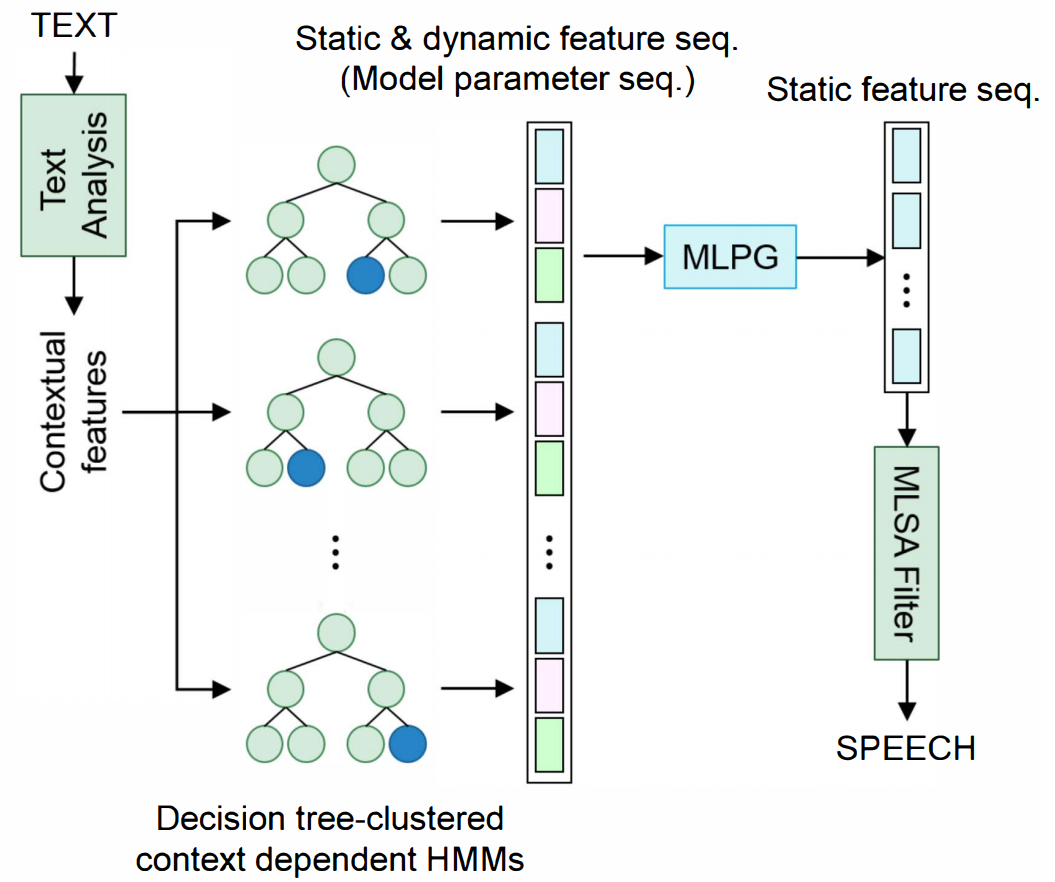
\includegraphics[width=\linewidth]{images/hmm_spss.png}
		\captionof{figure}{The general HMM-based TTS synthesis approach.}
		\label{hmm_spss_framework}
	\end{minipage}
	\hspace{.05\linewidth}
	\begin{minipage}{.45\linewidth}
		\centering
		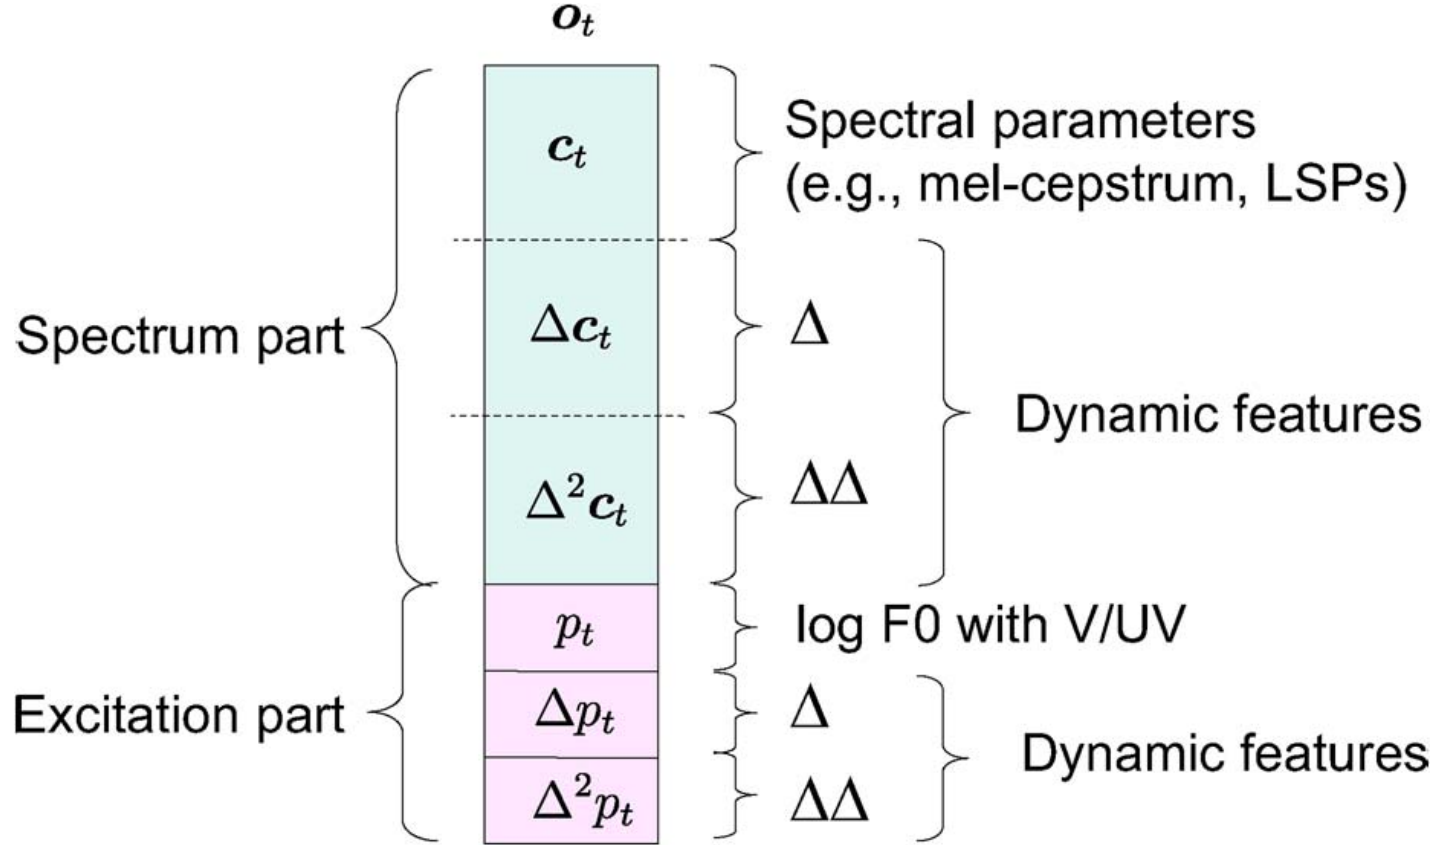
\includegraphics[width=\linewidth]{images/mlpg_features.png}
		\captionof{figure}{Dynamic and static features produced by the HMMs. F0 is the fundamental frequency and V/UV is the voicing flag.}
		\label{mlpg_features}
	\end{minipage}
\end{figure}

Improvements to this framework were later brought by feed-forward deep neural networks (DNN), as a result of progress in both hardware and software. \citep{SPSSDNN} proposes to replace entirely the decision tree-clustered HMMs in favor of a DNN. They argue for better data efficiency as the training set is no longer fragmented in different clusters of contexts\color{red}, and for a more powerful model?\color{black}. They demonstrate improvements over the speech quality with a number of parameters similar to that of the HMM-based approach. Their best model is a DNN with 4 layers of 256 units using a sigmoid activation function. Subjects assessing the quality of the generated audio samples report that the DNN-based models produces speech that sounds less muffled than that of the HMM-based models. Later researches corroborate these findings \citep{OnTheTrainingAspects}. \citep{Hashimoto-2015} additionally studies the effect of replacing MLPG with another DNN. The combinations of HMM/DNN and MLPG/DNN give rise to four possible frameworks, the novel ones being HMM+DNN and DNN+DNN\footnote{Note that since the two networks are consecutive in the framework, they can be considered a single network.}, while HMM+MLPG and DNN+MLPG are the frameworks described respectively in \citep{Tokuda-2013} and \citep{SPSSDNN}. Each DNN they use is 3 layers deep with 1024 units using a sigmoid activation function. MOS results confirm that DNN+MLPG is significantly better than HMM+MLPG. The DNN+DNN approach performs as well as HMM+MLPG while HMM+DNN is worse. In another experiment, they introduce a DNN before and after MLPG. While both approaches yield a MOS similar to DNN+MLPG, neither are statistically significantly better. \color{red} make this part nicer to read or maybe just remove it? Quid of the MOS? Mention DMDN?\color{black}

%\begin{wraptable}{r}{5.5cm}
%	\begin{tabular}{| l | c |}
%		\hline
%		Method & MOS \\
%		\hline
%		HMM+MLPG & 3.08 ($\pm$0.12) \\
%		HMM+DNN & 2.86 ($\pm$0.12) \\
%		\textbf{DNN+MLPG} & \textbf{3.53 ($\pm$0.12}) \\
%		DNN+DNN & 3.17 ($\pm$0.12) \\
%		\hline
%	\end{tabular}
%	\caption{MOS of the different methods explored in \citep{Hashimoto-2015}}
%	\label{hashimoto_results}
%\end{wraptable}

\citep{BDLSTMTTS} supports that RNNs make natural acoustic models as they are able to learn a compact representation of complex and long-span functions, better so than shallow architectures such as the decision trees used in HMM-based TTS. Furthermore, the internal state of RNNs makes the mapping from an input frame to output acoustic features no longer deterministic, allowing for more variety in the synthesized audio. As RNNs are fit to generate temporally consistent series, the static features can directly be determined by the acoustic model, alleviating the need for dynamic features and MLPG. The authors present two RNNs: Hybrid\_A with three feed-forward layers followed by one bidirectional (BDLSTM) layer and Hybrid\_B with two feed-forward layers followed by two BDLSTM layers. They argue that deeper structures of BDLSTM would worsen the performance due to imprecise gradient computation. They compare these networks against the HMM and DNN based approaches described previously, using objective and subjective measures. The objective measures are compared with the ground truth: log spectral distance (LSD), voiced/unvoiced (V/UV) error rate and fundamental frequency (F0) distortion in root mean squared error (RMSE). The subjective measure is a preference test where participants must choose between two audio samples of different models and have the option to select neither. Results are shown in figures \ref{dblstm_objective} and \ref{dblstm_subjective}. DNN\_A is 6 layers deep with 512 units per layer while DNN\_B is 3 layers deep with 1024 units per layer. These two networks perform very similarly. Hybrid\_B systematically performs better than the other approaches.

%3: Main advantage: long span and compact representation of complex functions. DTs are shallow. Not only memory but also internal hidden states which means non determinism wrt input states.
%3: Because RNN good for sequences -> direct prediction of same static features without dynamic
%4.1: Similar input features
%4.1: Using LSP and not MFCC
%4.1: Claim to be limited by depth
%4.2: Preference score

\begin{figure}[h]
	\centering
	\begin{minipage}{.45\linewidth}
		\centering
		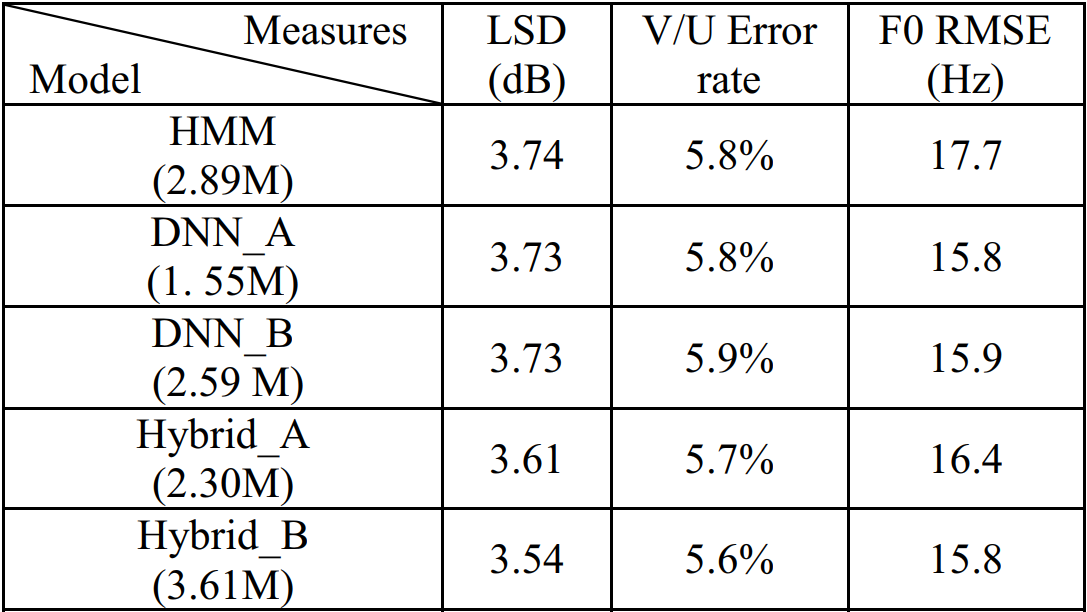
\includegraphics[width=\linewidth]{images/bdlstm_objective.png}
		\captionof{figure}{Performance of the different frameworks evaluated on objective measures. In parentheses are the number of parameters of each acoustic model.}
		\label{dblstm_objective}
	\end{minipage}
	\hspace{.05\linewidth}
	\begin{minipage}{.45\linewidth}
		\centering
		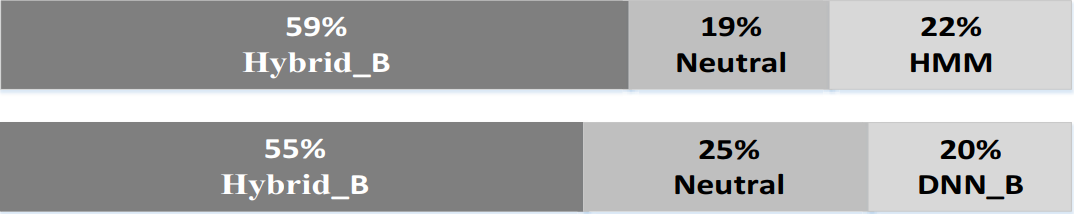
\includegraphics[width=\linewidth]{images/bdlstm_subjective.png}
		\captionof{figure}{Two by two comparisons of some of the frameworks in terms of preferences.}
		\label{dblstm_subjective}
	\end{minipage}
\end{figure}

Later, a substantial breakthrough in TTS is achieved with the coming of WaveNet \citep{WaveNet}. WaveNet is a deep convolutional neural network that, for a raw audio waveform, models the distribution of a single sample given all previous ones. It is thus possible to generate audio by predicting samples one at a time in an autoregressive fashion. WaveNet leverages stacks of one-dimensional dilated convolutions with a dilation factor increasing exponentially with the layer depth, which allows for a very large receptive field.
% causal convolutions which ensure that only the samples of previous timesteps are used to generate the sample of a given timestep. (Do we really care?)
The output is a categorical distribution (using a softmax layer) over sample values. For tractability reasons, the output signal is restricted to 256 values that correspond to a $\mu$-law quantization, which is invertible. The MOS resulting from one of the experiments suggests that there is no statistically significant degradation in the naturalness of speech quantized in this manner. The architecture of WaveNet comes with several non-trivial components, described in later sections of this document \color{red}link to the section\color{black}. On its own, a trained WaveNet generates sound alike the training data but without semantics. The network must be locally conditioned on linguistic contexts to achieve TTS synthesis. Furthermore, it allows for conditioning with respect to a vector constant at every timestep (global conditioning), which can be used to designate the speaker identity. The authors suggest that WaveNet is able to encode the embedding of several speakers seen in training with a shared internal representation. Speaker identities are given as a one-hot encoding. The audio generated by WaveNet requires no post-processing other than the inversion of the $\mu$-law. TTS with WaveNet does not exactly fit as an SPSS system considering that it does not produce clear intermediate acoustic features and instead serves as both a statistical model and a vocoder in a single pipeline. Performance scores are reported in Figure \ref{wavenet_results}. The parametric approach is an LSTM-based system while the other is an HMM-driven unit selection concatenative system (not detailed in this document). Notice how the results vary between US English and Mandarin Chinese, showing that TTS performance is not language agnostic. \color{red} recheck all the info on WaveNet later + F0??\color{black}

\begin{figure}[h]
	\centering
	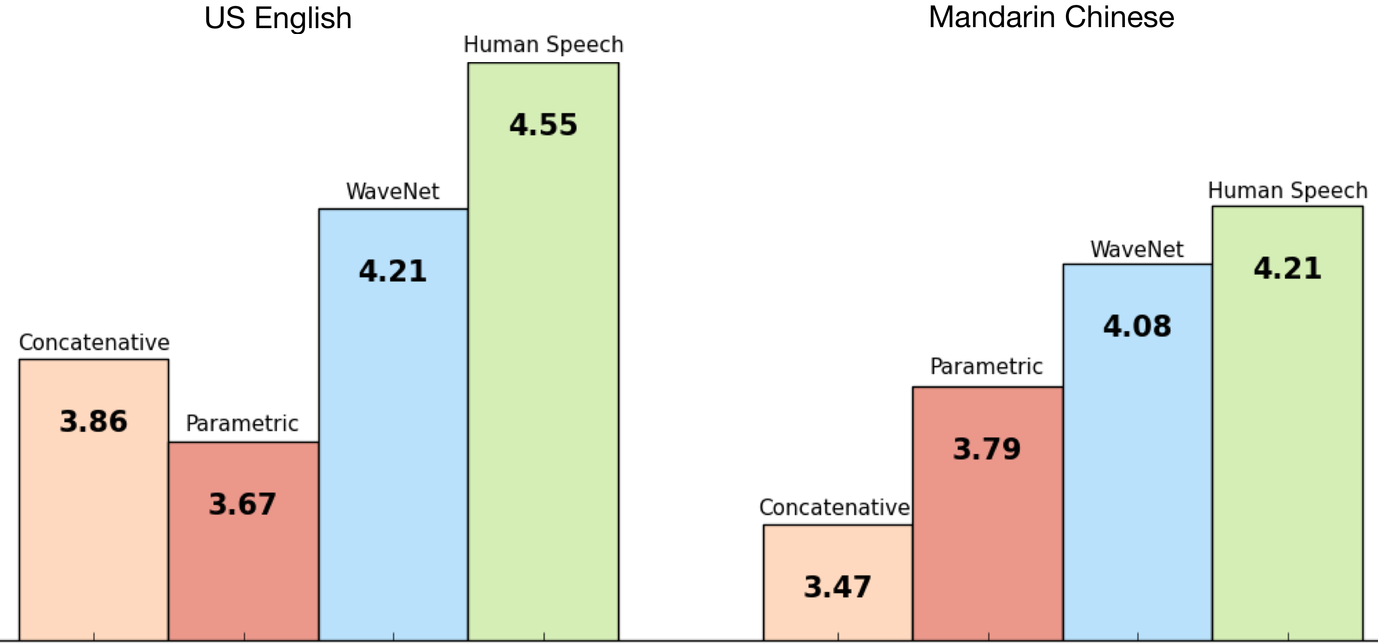
\includegraphics[width=.7\linewidth]{images/wavenet_results_chart.png}
	\caption{MOS of WaveNet's performance compared with a parametric and concatenative approach as well as with natural speech.}
	\label{wavenet_results}
\end{figure}

%1 SOTA TTS \\
%2.1 Dilated causal convolutions \\
%2.2 u-law \\
%2.3 Gated activations - Relu  \\
%2.4 Residual \\
%2.5 Condition on speaker identity (one hot) + local conditioning \\
%2.6 Context stack \\
%3.1 All speakers embedded in WaveNet and sharing internal representation
%Annex: Raw audio gen with no postprocessing \\
%Annex DV: Type of features, direct sampling, white noise


Deep Voice \citep{DeepVoice1} proposes a fully neural TTS framework that exploits WaveNet among other deep architectures. Deep Voice stands out by making use of only a few intermediate features: phonemes with stress annotations, phoneme durations,
and F0. This has the advantage of making the framework easily transferable to new domains with little engineering effort as complex linguistic features need not be derived. The neural networks intervening in Deep Voice are: a grapheme-to-phoneme model that converts text to phonemes, a segmentation model that aligns a sequence of phonemes to an audio segment, a phoneme duration model that predicts the duration of each phoneme at generation time, a fundamental frequency model that predicts the V/UV flag with F0 values for voiced parts and finally, WaveNet which acts as an audio synthesis model. In all the works we presented previously, only the audio synthesis model was not manually engineered. While others have researched the use of neural networks for some of these components, Deep Voice is the first to simultaneously employ them all in a single framework. However, the grapheme-to-phoneme model is only used as a fallback for words not present in a phoneme dictionary. The roles and interactions of these components at training and inference time are shown in figure \ref{deep_voice_1_arch}. Deep Voice also improves on the inference time of WaveNet, with a speedup of up to 400. This allows for real-time or near real-time execution, with a tunable speed/quality trade-off. Deep Voice does not yield state of the art results but instead serves as groundwork for future researches. \color{red} discuss results \color{black}.

\begin{figure}[h]
	\centering
	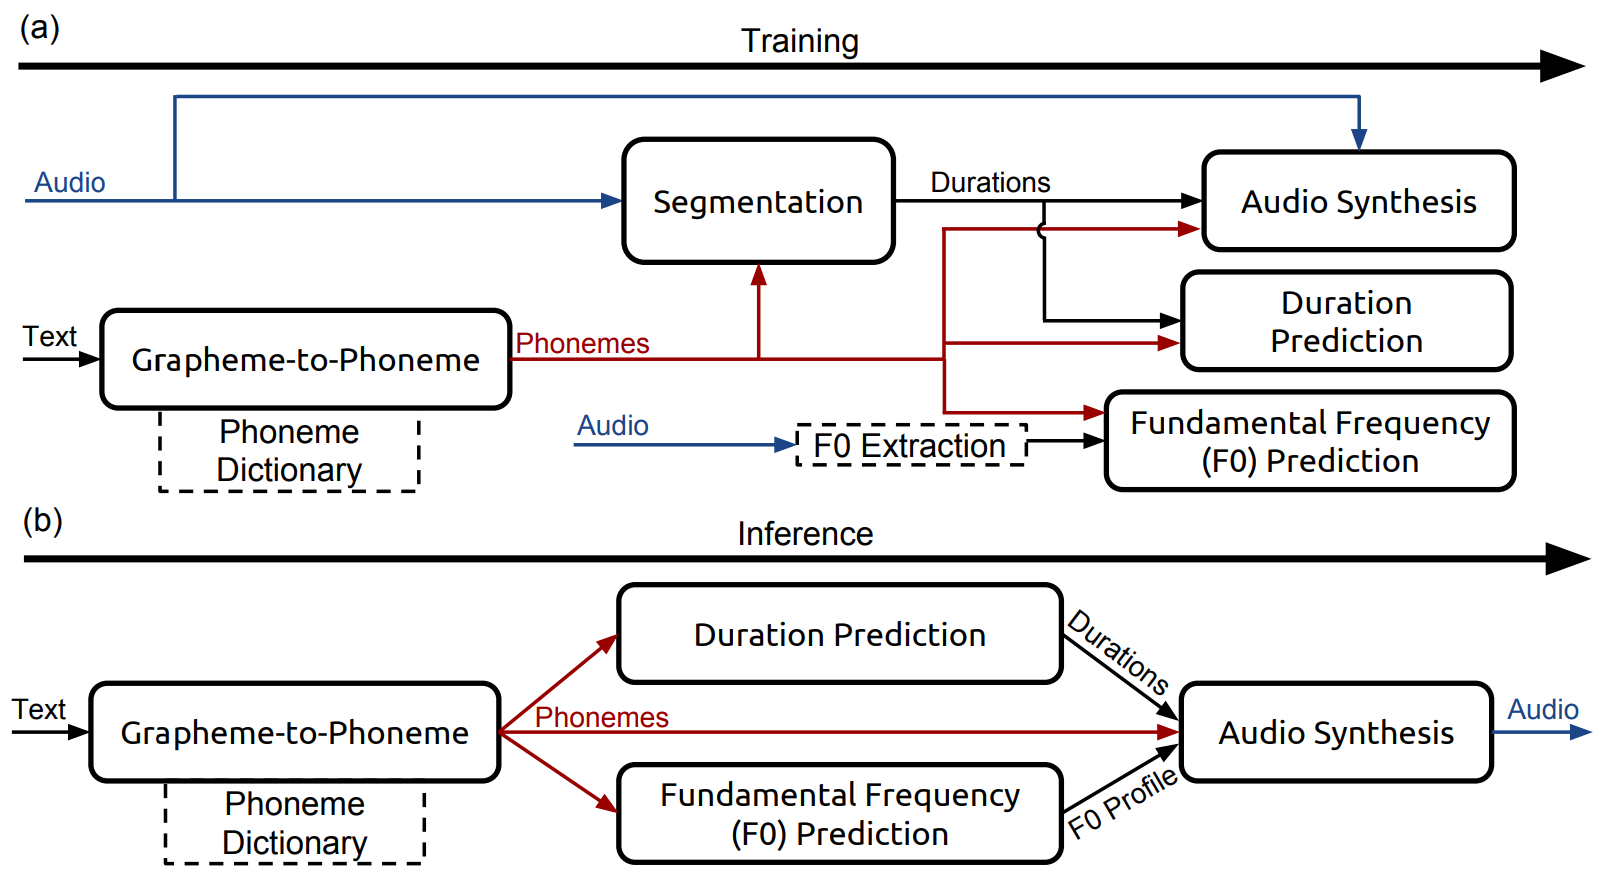
\includegraphics[width=.8\linewidth]{images/deep_voice_1_arch.png}
	\caption{The training (a) and inference (b) procedure of Deep Voice. On the left of the image are the inputs, on the right are the outputs. Note that the segmentation model is only used for training.}
	\label{deep_voice_1_arch}
\end{figure}

% Up to 400x speedup on WaveNet
% Some previous research already use models to generate textual features
% No words with multiple pronunciations
% Natural MOS score when using ground truth F0 and durations
% Near real-time (accuracy/speed tradeoff)
% No diff when using original WaveNet

\color{red}
Skipping the Deep Voice 2 \& 3papers. I'll see later whether or not I should include them
\color{black}

Published approximately at the same time, Tacotron \citep{Tacotron1} is a sequence-to-sequence model that produces a spectrogram from a sequence of characters alone, further reducing the need for domain expertise. An audio waveform can be estimated from the spectrogram using the Griffin-Lin algorithm. Tacotron is also built fully with neural networks and is trained in an end-to-end fashion. It uses an encoder-decoder architecture where, at each step, the decoder operates on a weighted sum of the encoder outputs. This mechanism described in \citep{Attention} lets the network decide which steps of the input sequence are important with respect to each steps of the output sequence. Tacotron achieves a MOS of 3.85 on a US English dataset, which is more than the 3.69 score obtained in the parametric approach of \citep{LSTM-RNN} but less than the 4.09 score obtained by the concatenative approach of \citep{ConcatenativeGoogle}. The authors mention that Tacotron is merely a step towards a better framework. By the end of 2017, Tacotron 2 is published \citep{Tacotron2}. The architecture of Tacotron 2 remains that of an encoder-decoder with attention although several changes to the types of layers are made. The main difference with Tacotron is the addition of a modified WaveNet for vocoder. On the same dataset, Tacotron 2 achieves a MOS of 4.53 compared to 4.58 for human speech (the difference is not statistically significant), achieving the all-time highest MOS. In a preference study, Tacotron 2 was found to be only slightly less preferred on average than ground truth samples. The ratings from that study are shown in figure 

\begin{figure}[h]
	\centering
	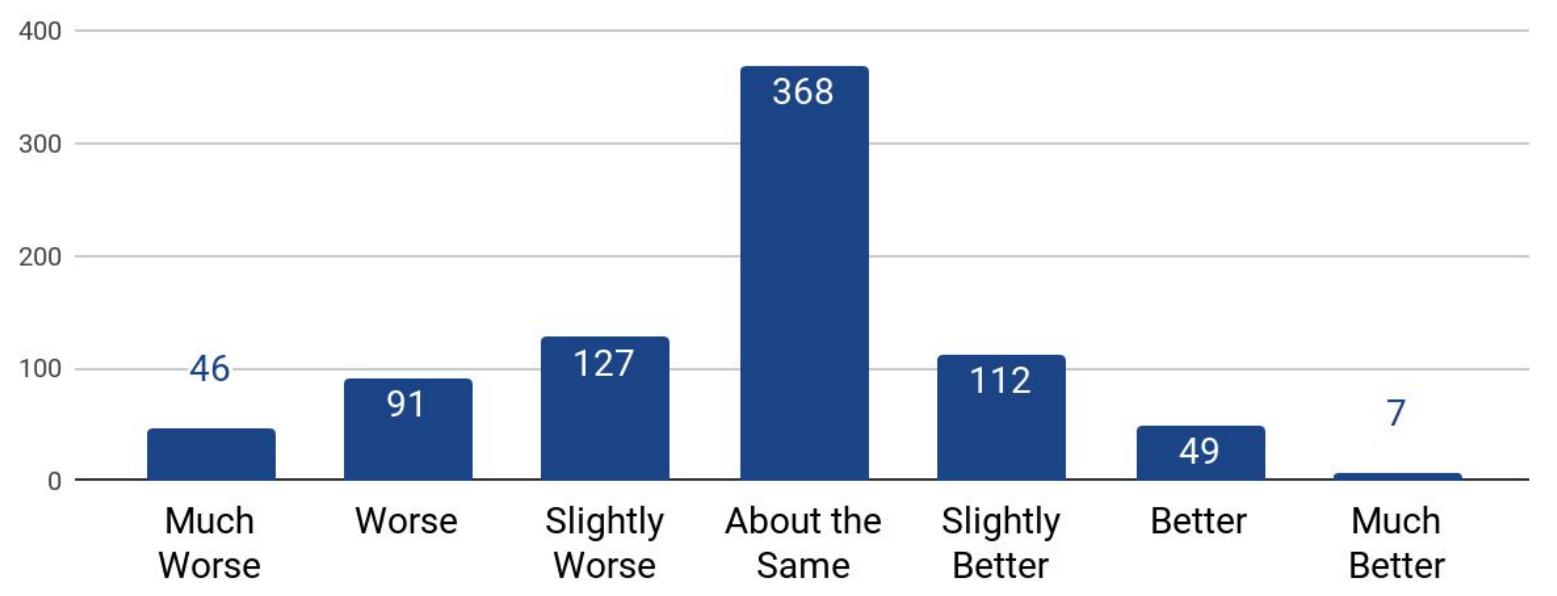
\includegraphics[width=.8\linewidth]{images/tacotron2_results.png}
	\caption{Preference ratings between Tacotron 2 and ground truth samples. 800 ratings on 100 items. The labels are expressed with respect to Tacotron 2.}
	\label{tacotron2_results}
\end{figure}


\color{red}
Few samples

SV2TTS

Extensions?

Link audio samples for everything where available
\color{black}


\section{Transfer Learning from Speaker Verification to Multispeaker Text-To-Speech Synthesis}
To achieve our goal of real-time voice cloning, we reproduce \citep{SV2TTS} (referred as SV2TTS throughout this document). It describes an approach to multispeaker speech synthesis. A multispeaker speech synthesis framework is able to generate speech from text using different voices. This set of voices may be encoded into the model or be external to the model. In the first case, 

\color{red}This should come earlier\color{black}

The approach used in SV2TTS is to build three models that are trained separately:
\begin{itemize}
	\item A speaker encoder that derives an embedding from the short utterance of a single speaker. The embedding is a meaningful representation of the voice of the speaker, such that similar voices are close in latent space. This model is described in \citep{GE2E} (referred as GE2E throughout this document) and \citep{TE2E}.
	\item A synthesizer that, conditioned on the embedding of a speaker, generates speech features from a given text. This model is the popular Tacotron 2 \citep{Tacotron2} without WaveNet. The generated features cannot trivially be converted to an audio waveform. 
	\item A vocoder that infers an audio waveform from the intermediate features generated by the synthesizer. The authors used WaveNet \citep{WaveNet} as vocoder, effectively reusing the entire Tacotron 2 framework.
\end{itemize}

In the future, we will refer to these three models as respectively the encoder, the synthesizer and the vocoder. At inference time, the encoder is fed a reference utterance of the speaker to clone. It generates an embedding that is fed to the synthesizer, along with a selected text to generate. Finally, the vocoder takes the output of the synthesizer to generate the speech waveform. 

\begin{figure}[t]
	\centering
	\caption{Model overview.  Each of the three components are trained independently.}
	\label{fig.model_overview}
\end{figure}



Note that all models are interchangeable provided that they perform the same task. In particular, vanilla WaveNet is extremely slow for inference. Several later papers brought improvements on that aspect to bring the generation near real-time or faster than real-time, e.g. \citep{ParallelWaveNet}, \citep{FastWaveNet}. Note that in this context, real-time is achieved when the generation time is shorter than or equal to the duration of the generated audio. In our implementation, the vocoder used is based on WaveRNN \citep{WaveRNN}.





\color{red}
- audio samples \\
encoder (or any):- a word about digital audio  \\
encoder: - meaning of the paper title  \\
synth: - the need of intermediate audio features  \\
synth: - advantages of conditioning on embedding rather than \\
\color{black}


\clearpage
\bibliographystyle{plainnat}
\bibliography{references} 




















%$$\Leftrightarrow h_b(x) =
%\left\{\begin{array}{lll}
%0 & if & P(y = 0 | x) > P(y = 1 | x)\\ 
%1 & else &
%\end{array}\right.$$



%\begin{figure}[h]
%	\centering
%	\includegraphics[width=16cm]{image.png}
%	\caption{caption}
%	\label{label}
%\end{figure}



%\begin{figure}[h]
%	\centering
%	\captionsetup{justification=centering}
%	\hspace{-1cm}
%	\subfigure{\includegraphics[height=5cm]{image.png}}
%	\subfigure{\includegraphics[height=5cm]{image.png}}
%	\hspace{-1cm}
%	\caption{caption}
%	\label{label}
%\end{figure}


%\begin{center}
%	\begin{tabular}{|r|ccc|ccc|}
%		\hline
%		& \multicolumn{6}{c|}{Validation set}\\
%		\hline
%		& \multicolumn{3}{c|}{Valid images (3126)} & \multicolumn{3}{c|}{Invalid images (3126)} \\
%		\hline
%		& Correct & Unclassified & Incorrect & Correct & Unclassified & Incorrect \\
%		\hline
%		Reduced & 94.98\% & 3.07\% & 1.95\% & 95.27\% & 2.91\% & 1.82\% \\
%		Lenet & 98.08\% & 0.74\% & 1.18\% & 97.86\% & 0.96\% & 1.18\% \\
%		\hline
%	\end{tabular}
%	
%	\vspace{0.5cm}
%	  
%	\begin{tabular}{|r|ccc|ccc|}
%		\hline
%		& \multicolumn{6}{c|}{Test set}\\
%		\hline
%		& \multicolumn{3}{c|}{Valid images (999)} & \multicolumn{3}{c|}{Invalid images (74)} \\
%		\hline
%		& Correct & Unclassified & Incorrect & Correct & Unclassified & Incorrect \\
%		\hline
%		Reduced& 94.29\% & 3.70\% & 2.00\% & 95.95\% & 4.05\% & 0.00\%  \\
%		Lenet & 96.90\% & 1.30\% & 1.80\% & 97.30\% & 1.35\% & 1.35\% \\
%		\hline
%	\end{tabular}
%\end{center}


\end{document}













































































































